\chapter{Event Selection}\label{chapt:event_selection}
 
This work was aiming to reconstruct the $t\bar{t}$ pair in the dilepton decay channel, or
$t\bar{t} \to W^{+}b\,W^{-}\bar{b} \to \bar{l}b\,l\bar{b}$. Thus the aim is to 
look for the event in the detector with two leptons of the different sign and two jets. The 
neutrino can't be measured directly, their presence is reflected in the non-zero transverse
missing energy $E_{T}^{miss}$. The lowest branching ratio of the dileptonic decay channel
($BR \simeq 4.8\%$) is countervailed by a a precise lepton reconstruction, which can reduce
the fraction of the background events to larger extend.

The dataset used for this measurement was collected over the full 2012 run period of the LHC
by the CMS detector with a collected integrated luminosity of $\mathcal{L} = 19.7 \pm 0.5 \textrm{pb}^{-1}$.

This chapter gives an overview of the $t\bar{t}$ final state objects reconstruction and selection. The 
procedures are based on the CMS Top-Quark-Physics-Analysis group recommendations \cite{TopPAGreco}.
The full chain of event selection are described and the details of each component reconstruction are given. 
Resulting event yields are represented in the control distributions, showing the data, simulated signal and backgrounds.

\section{Event cleaning and Pile-Up treatment}

In a very harsh and busy environment which the LHC collisions provide for the CMS detector, it is necessary to make an event 
cleaning. For this sake the \textit{filters} are used.

One of the filter removes \textit{beam scraping} events which have a large background from the beam remnants. This filter accepts 
the events with maximum 10 reconstructed tracks or those with more than 10 tracks, but at least quarter of them should have
high quality.

The phenomenon that one collision may contain several points of hadronic interaction, or \textit{primary verteces}, is called \textit{pile-up}. 
This effect challenges the data analysis thus needs a separate treatment. 

First all the verteces in the event are reconstructed.
Tracks which appear to originate from the same point in space are clustered and afterwards the position of the vertex if fitted using those tracks \cite{TrackPerf}.

After the vertex reconstruction the second filter used for this analysis selects the events with at least one "good" primary vertex.
This means that the number of associated tracks should be larger then 4 and a vertex should be positioned centrally in the detector
\footnote{Only the events with the vertex position $|z| < \textrm{24 cm}$ and $|\rho| < \textrm{2 cm}$ are accepted. All the coordinates
are given with respect to the CMS coordinate system (see sec.\label{sec:CMS} )}. To overcome the pile-up the primary vertex with the 
largest sum of transverse momenta squared ($p_{T}^{2}$) of the associated tracks is taken for further analysis.

The events with \textit{anomalous noise} from calorimeters are removed by the third filter.

\section{Trigger selection}

All the data flow in the CMS detector is reduced by triggers based on the physical requirements (see sec. \ref{sec:trig}).
The HLT triggers provide a selection which sorts the data by the processes which are taking place in the events. Thereby
a choice of a trigger which selected the events is already easing the task of selecting the correct physical process from
all the recorded data.

The events for this work were selected using several dileptonic HLTs which require at least two leptons (electrons or muons)
with the momenta larger than 15 GeV for one of them and 8 GeV for another. To identify a muon the triggers use the information
from the inner tracker and muon system. An electron is identified from the tracker and calorimeter information and additionally
has to fulfill a very loose isolation criterion. The details on the trigger paths used for this analysis are given in the
Appendix !!!.

As all of the data recorded is accepted by some HLT trigger, the determination of a particular trigger efficiency is determined with 
respect to another independent trigger. To calculate the dileptonic trigger efficiencies the triggers based on $E_{T}^{miss}$ selection
were taken as a reference.

\section{Particle Flow Concept}\label{sec:PF}

All the objects in $t\bar{t}$ dileptonic final state were reconstructed making use of \textit{Particle Flow} (PF)
algorithm \cite{Beaudette:2014cea}. In other words each particle or jet is identified exploiting the information from all parts
of the detector instead of using only one dedicated detector sector. The algorithm relies on an efficient track reconstruction,
clustering algorithm in wich is able to distinguish overlapping showers and on the efficient linking procedure to connect 
the signals from different sub-detectors.

A simplistic description of the reconstruction with the PF algorithm can be given as follows \cite{Beaudette:2014cea}.

\begin{itemize}
 \item [--] Muons are identified beforehand to exclude overlapping with the charged hadrons. Their tracks are extrapolated
 from tracker to calorimeter clusters and to the muon systems. An example of muon reconstruction using particle flow algorithm is 
 shown on the figure \ref{fig:PFmuons}. The clusters in calorimeter and tracks in the tracker which the muons are assigned to
 do not enter the further objects identification process.
 %
 \item [--] Charged hadrons are reconstructed from the tracks which after the extrapolation to the HCAL region fall within the boundaries
 of one or more calorimeter clusters. Analogically to the tracks used for muon identification, tracks associated to the charged 
 hadrons do not enter any further particle reconstruction.
 %
 \item [--] Electrons have to be reconstructed taking into account not only the tracks and ECAL deposits matching to them, but also
 adding the photons from the frequent Bremsstrahlung.
 %
 \item [--] The remaining ECAL clusters are assigned to photons, and the one from HCAL - to the neutral hadrons
\end{itemize}

\begin{figure}[t]
  \centering
  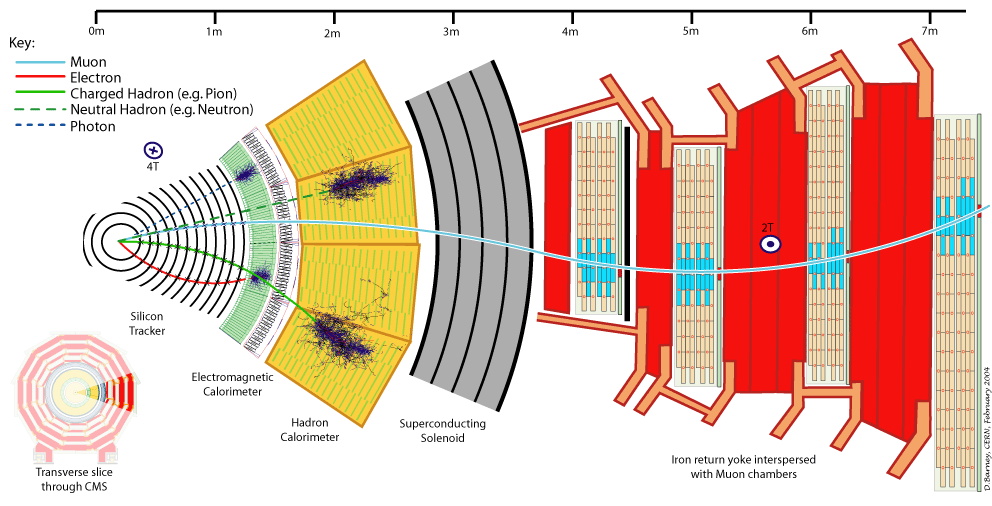
\includegraphics[width=1.0\textwidth]{04_event_reconstruction/plots/CMS_Slice.png}
  \caption{Track reconstruction using different sub-detector information in combination in Particle Flow algorithm. An actual
  muon track is shown with a curved blue line, an electron track is red and a charged hadron is solid green.}
  \label{fig:PFmuons}
\end{figure}

The resulting list of particles is used for further jet and missing transverse energy ($E_{T}^{miss}$) construction. 

The performance of the algorithm was studied with the simulated events \cite{CMS-PAS-PFT-09-001}. Particularly the jet energy
resolution gain reaches factor 3 for a low transverse momentum region. Furthermore, the angular resolution is improved by factor 2-3.

A more detailed description of each object reconstruction relevant for this analysis is given in the following sections of this chapter.
A complete overview of the PF algorithm can be found in \cite{CMS-PAS-PFT-09-001}. 

\section{Lepton reconstruction and selection}

The presence of two leptons, electrons or muons, is required for this analysis. Their reconstruction
differs a lot due to a huge mass distinction. Thus, the reconstruction of leptons and muons is discussed separately.

\subsection{Muons reconstruction}

As it was discussed in section \ref{sec:CMS}, the CMS experiment has a well established setup for the muon reconstruction.
Muons are the only particles expected to appear in the muon sub-detector system, thus their identification is unambiguous.
Three techniques of muon reconstruction were implemented:

\begin{itemize}
 \item [--] \textit{Standalone}: muons are reconstructed using the information from the muon system only. As 
 this part of the detector provides a tracking information, a complete set of physical properties needed for the further
 analysis is recorded.
 
 \item [--] \textit{Tracker}: the tracks, reconstructed in the tracking detector only, are assigned as muons in case they 
 match at least one hit in the muon sub-detector. 
 
 \item [--] \textit{Global}: the muons are reconstructed using 
 the combined fit of tracks from the muon system and from the inner tracker.
\end{itemize}

Only the global or tracker muons were used for this analysis. It is more efficient to use the tracker algorithm to reconstruct
low-momentum muons, but it suffers a lot from the presence of a large number of other particles. The global muons with small momenta
are dominantly using the tracking detector information for the reconstruction, while starting from $p_{T} \sim \textrm{200 GeV}$
the muon system data plays a significant role.

\subsection{Electrons reconstruction}

To reconstruct the electrons a combined information from the tracking detector and ECAL was used \cite{CMS-PAS-EGM-10-004}. The energy
deposits in the ECAL are grouped into superclusters\footnote{A \textit{supercluster} is  a group of one or more associated clusters 
of energy deposits in the ECAL. It is constructed taking into account its characteristic narrow width in the pseudorapidity $\eta$
and its characteristic spread in $\phi$ due to the bending in the magnetic field of electrons radiating in the tracker material.} 
with transverse energy $E_{T} > \textrm{4 GeV}$ and fitted to the tracks in the tracking detector \cite{GSF_Electron_Reconstruction_CMS}.

For a better quality of the tracks a restriction on the impact parameter\footnote{An \textit{impact parameter} $d_{xy}$ of the track is a minimum
distance of the track to the primary vertex in the transverse $x-y$ plane.} $|d_{xy}| < 0.4 mm$ is applied. A maximum one hit in the inner tracker
which is positioned close to the track, but not reconstructed, is allowed for the electron candidate.

On top of the mentioned conditions, a multivariate analysis (MVA) is performed to reduce the number of misidentified electrons.

\subsection{Lepton selection and isolation}

Only the events which contain at least two leptons (electrons or muons) with a minimum transverse momentum $p_{T}$ of 20 GeV reconstructed
in central detector part $|\eta| \leq 2.4$ are accepted for the further analysis.

To distinguish leptons from hard processes (like a $W^{\pm}$ decay), or \textit{prompt leptons}, from the misidentified charged hadrons 
and leptons from the jets, an \textit{isolation} criterion is required. The former usually don't overlap with jets, while the latter should
fly in the same direction and be located in a close vicinity of a jet. This distinction is a basis for the isolation. An energy in a cone 
around a lepton (not counting the lepton energy itself) is calculated. That is the definition of a combined isolation:

\begin{equation}
 I_{comb} = I_{tracker} + I_{ECAL} + I_{HCAL} = \sum E_{photons} + \sum E_{hadrons}
\end{equation}

The combined isolation $I_{comb}$ divided by the lepton transverse momentum $p_{T}(l)$ is the relative isolation used as a discriminant value:

\begin{equation}
 I_{rel} = \frac{I_{comb}}{p_{T}(l)}
\end{equation}

Leptons with the $I_{rel} \leq 0.15$ in the cone $\Delta R = \sqrt{\Delta\eta^{2} + \Delta\phi^{2}} = 0.3$ are selected.

\subsection{Lepton pair selection}

The $t\bar{t}$ decay final state has two oppositely charged leptons, while the selected events may contain three or more leptons.
Out of all the leptons in the event, only the pair of opposite sign tracks with the maximum total transverse momentum $p_{T}(l\bar{l})$
is selected. After this step the event is tagged with the $t\bar{t}$ decay channel -- $ee$, $e\mu$ or $\mu\mu$.

To minimize the fraction of the Drell-Yan low-mass resonances only the lepton pairs with the masses higher then 20 GeV are accepted. 

The same flavour final states ($ee$ and $\mu\mu$) are highly contaminated by the $Z/\gamma * \to ee/\mu\mu$ processes. To lower this effect
the restriction on the mass window of the lepton pair system $\textrm{76 GeV} \leq m(l\bar{l}) \leq \textrm{106 GeV}$ is applied which removes  
the mass peak of the $Z-$boson resonance at $\textrm{91 GeV}$. This condition is only required for the $ee$- and $\mu\mu$-tagged events.

% \subsection{Lepton Isolation}
%
% \section{Jets}
% \subsection{Jet Finder Algorithm}
% \subsection{Jet selection}
% \subsection{b-Jets identification}
% 
% 
% \section{Missing Transverse Energy}
% 
% \section{Control Distributions}